\documentclass[a4paper,12pt]{article}

\usepackage{superpack2015}
\usepackage{tkz-fct}
\usepackage{lscape}

\usepackage[heightrounded]{geometry}	% heightrounded permet d'afficher les footers correctement
\geometry{hmargin=0.5cm,vmargin=1.5cm}

\setlength{\columnseprule}{0.5pt}		% Ligne séparatrice milieu document
\setlength{\columnsep}{50pt}			% Espace de chaque côté de la ligne
\setlength{\headsep}{15pt}
\addtolength{\textheight}{20pt}
%\setlength{\textwidth}{770pt}
%\setlength{\hoffset}{20pt}

\classichf
	% Nom du style
	{activites}
	% Hauteur sous header
	% 14.5pt si une ligne (1 \baselineskip)
	% 29.0pt si deux lignes (2 \baselineskip)
	{14.5pt}
	% Head
	{}
	{\textbf{Activités : Généralités sur les fonctions}}
	{}
	% Foot
	{}
	{}
	{}

%\usepackage{showframe}
%\usepackage{layout}

\begin{document}
\pagestyle{activites}	%\thispagestyle{premierepage} pour isoler des styles de pages

\setcounter{activite}{-1}
\activite hauteur d'eau du Gardon d'Alès le 28/10/2015\\
On donne ci-dessous la hauteur d'eau du Gardon d'Alès en mètres représentée en fonction de l'heure de la journée du mercredi 28 octobre 2015\footnote{source~: \url{http://www.vigicrues.ecologie.gouv.fr}}. On appellera cette fonction $h$.
\begin{center}
	\exercice Reprenons la fonction $h$ évoquée dans l'activité
\vspace*{-1em}
\begin{center}
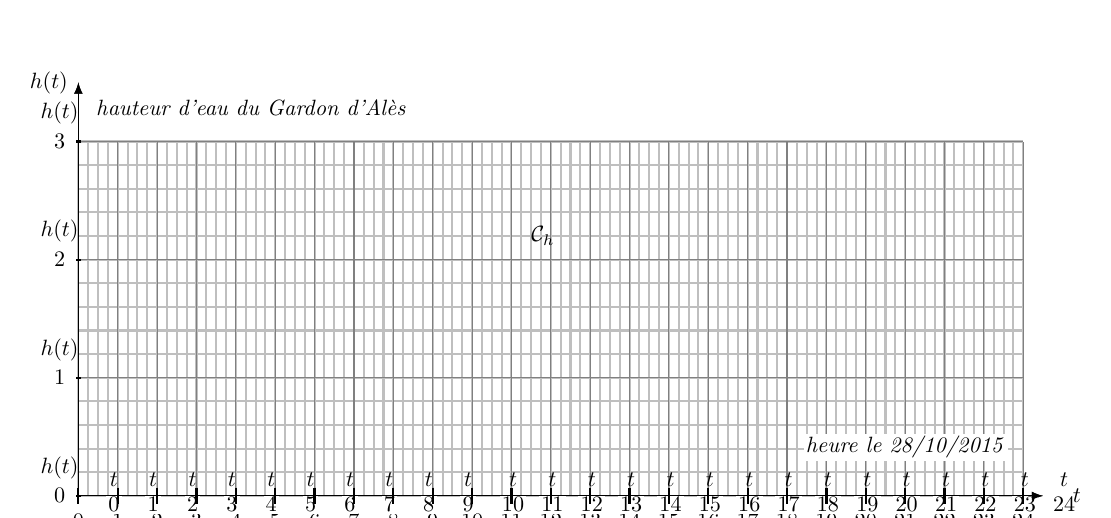
\begin{tikzpicture}[scale=0.5,yscale=3,every node/.style={scale=0.8}]
\tkzInit[xmax=24,xstep=1,ymax=3,ystep=1]
\tkzGrid[sub,
		subxstep=0.25,
		color=gray]
\tkzLabelX
\tkzDrawX[label={\textit{heure le 28/10/2015}},above left=18pt,fill=white]
\tkzLabelY
\tkzDrawY[label={\textit{hauteur d'eau du Gardon d'Al\`es}},below right=8pt]
\draw plot[smooth] file {ales.table.suite};
\tkzAxeX[label=$t$,right=10pt]
\tkzAxeY[label=$h(t)$]
\tkzText(11.8,2.2){$\mathcal{C}_{h}$}
\end{tikzpicture}
\end{center}

\begin{enumerate}
	\item Résoudre graphiquement $h(t) > 2$.
	\item Déterminer graphiquement les antécédents de $2$ par $h$.
	\item Déterminer graphiquement $h(22)$.
	\item Déterminer graphiquement le maximum de la fonction $h$ et la valeur de $t$ pour laquelle on l'obtient.
	\item Déterminer graphiquement les valeurs de~$t$ pour lesquelles la fonction~$h$ est croissante et celles où la fonction~$h$ est décroissante.
	\item Exprimer les réponses de la question précédente sous forme d'intervalles de valeurs de $t$.
	\item Pour chacune des questions précédentes, exprimer en langage courant ce qui est demandé.
	\item Répondre maintenant aux questions de 1. à \addtocounter{enumi}{-2}\theenumi \addtocounter{enumi}{2}.
\end{enumerate}
\end{center}

\vspace*{\stretch{1}}

\begin{enumerate}
	\item Traduire en langage courant les phrases suivantes :
\end{enumerate}

\begin{tabularx}{0.92\linewidth}{|p{0.02\linewidth}||p{0.42\linewidth}|p{0.42\linewidth}@{\parbox[c][2.5em][c]{0.4\textwidth}{}}|}
\hline
~ & \hspace*{1.7cm} Langage mathématique 			& \hspace*{2.3cm} Langage courant		\\ \hline
a. & $h(18) = 2$									& À 18h, la hauteur d'eau était de $2m$.\\ \hline
b. & L'image de $9$ par $h$ est $0,6$.				& À 9h, la hauteur d'eau \ldots			\\ \hline
c. & Quels sont les antécédents de $1,6$ par $h$~?	& À quelle heure \ldots ?					\\ \hline
d. & Le maximum de la fonction $h$ est $2,7$.		&										\\ \hline
e. & Si $12\text{h}15 < t < 18h$ alors $h(t) > 2$.	& Entre $12\text{h}15$ et $18\text{h}$ \ldots \\ \hline
f. & $h$ est strictement décroissante sur $[14;22]$& 										\\ \hline
\end{tabularx}

\vspace*{\stretch{1}}

\begin{enumerate}
	\setcounter{enumi}{1}
	\item Traduire en langage mathématiques les phrases suivantes :
\end{enumerate}

\begin{tabularx}{0.92\linewidth}{|p{0.02\linewidth}||p{0.42\linewidth}|p{0.42\linewidth}@{\parbox[c][2.5em][c]{0.4\textwidth}{}}|}
\hline
~  & \hspace*{2.3cm} Langage courant	 				&  \hspace*{1.7cm} Langage mathématique				\\ \hline
a. & À $9$h, la hauteur d'eau était de $60~cm$.			& 									\\ \hline
b. & À quelle heure la hauteur d'eau était de $1,8m$~?	& 									\\ \hline
c. & Quels sont les antécédents de $1,6$ par $h$~?		&									\\ \hline
d. & La hauteur d'eau minimale est de $45cm$.			& 									\\ \hline
e. & Entre $10$h$15$ et $22$h la hauteur d'eau est supérieure à $1m40$.	& 					\\ \hline
f. & Entre $9$h et $13$h$30$, le niveau de l'eau monte.	& \\ \hline
\end{tabularx}

\vspace*{\stretch{1}}

%\begin{longtable}{| p{0.2\linewidth} | p{0.2\linewidth} |}
%\caption{Titre du tableau}
%\hline
%ligne 1 colonne 1 & ligne 1 colonne 2 \\
%…
%\end{longtable}

\end{document}


%
%%\exercicebareme{4}
%\exercicebareme{6}
%\exercicebareme{10}
%\exerciceunpoint
%\exercicebonus
%\FIN
%\BONNESVACANCES
%\BONCOURAGE
%\hrulefill